\documentclass[oneside, 11pt]{article}

\usepackage[T1]{fontenc}
\usepackage[utf8]{inputenc}
\usepackage[english]{babel}

\usepackage{fouriernc}
\usepackage[detect-all, binary-units, separate-uncertainty=true,
            per-mode=symbol, retain-explicit-plus, retain-unity-mantissa=false]{siunitx}

\usepackage{setspace}
\setstretch{1.2}

\setlength{\parskip}{\smallskipamount}
\setlength{\parindent}{0pt}

\usepackage[headheight=14pt]{geometry}
\geometry{marginparwidth=0.5cm, verbose, a4paper, tmargin=3cm, bmargin=3cm,
          lmargin=2cm, rmargin=2cm}

\usepackage{float}

\usepackage[fleqn]{amsmath}
\numberwithin{equation}{section}
\numberwithin{figure}{section}

\usepackage{graphicx}
\graphicspath{{images/}{../../../images/}}

\usepackage{tikz}
\usetikzlibrary{shapes}
\usetikzlibrary{plotmarks}

\newcounter{Exercise}
\setcounter{Exercise}{1}
\usepackage{xcolor}
\definecolor{shadecolor}{gray}{0.9}
\usepackage{framed}
\usepackage{caption}

\usepackage{url}


\usepackage{fancyhdr}
\pagestyle{fancy}
\fancyhf{}
\rhead{\thepage}
\renewcommand{\footrulewidth}{0pt}
\renewcommand{\headrulewidth}{0pt}

\fancypagestyle{firststyle}
{
    \fancyhf{}
    \rhead{\thepage}
    \cfoot{
\includegraphics[height=30pt]{HiSPARClogo}}
    \rfoot{
\includegraphics[height=25pt]{CCbysa}}
    \lfoot{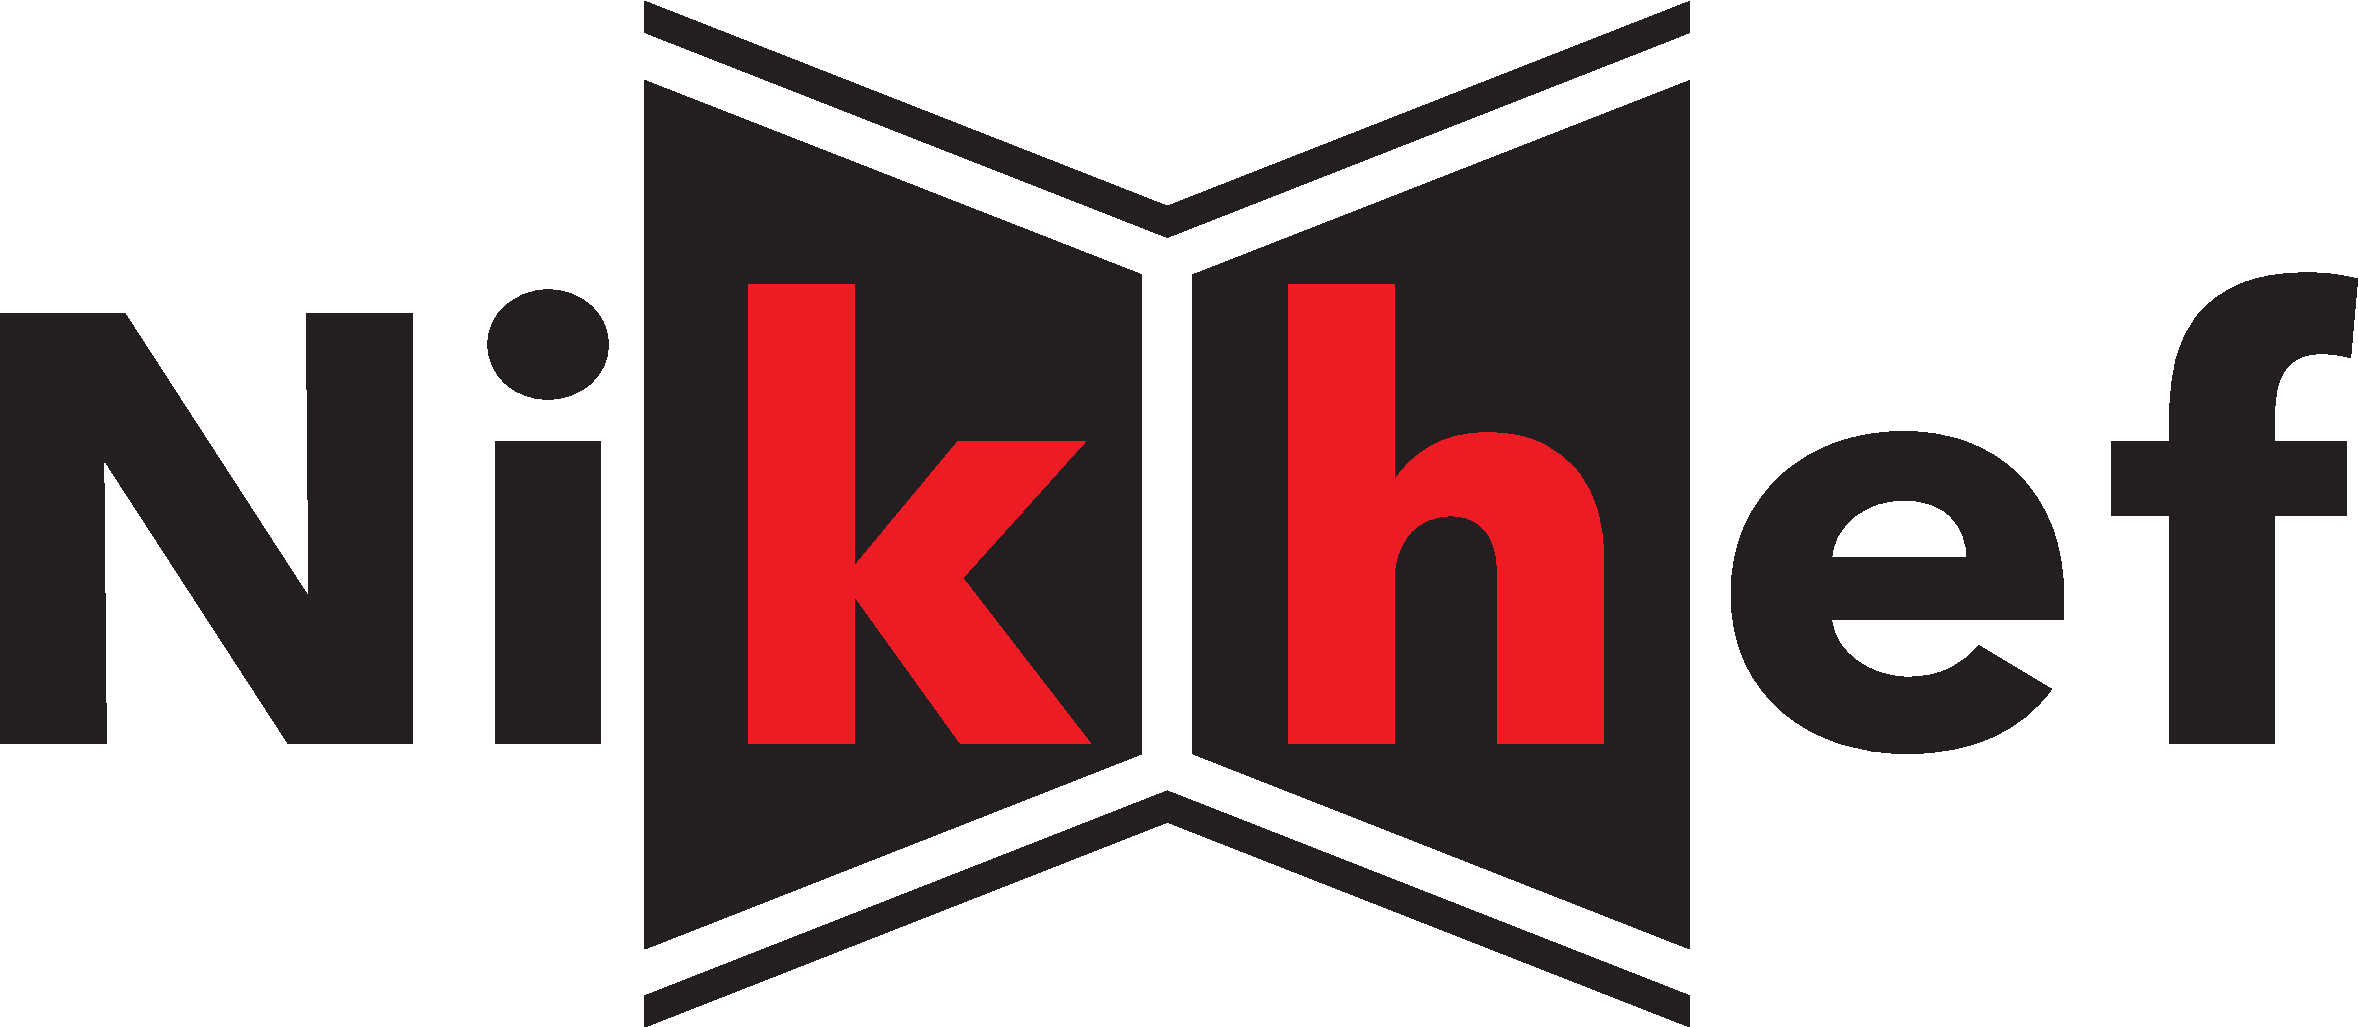
\includegraphics[height=30pt]{NIKHEFlogo}}
    \renewcommand{\footskip}{50pt}
    \renewcommand{\footrulewidth}{0.1pt}
    \renewcommand{\headrulewidth}{0pt}
}

\newcommand{\figref}[1]{Figuur~\ref{#1}}

\newcommand{\hisparc}{\textsmaller{HiSPARC}\xspace}
\newcommand{\kascade}{\textsmaller{KASCADE}\xspace}
\newcommand{\sapphire}{\textsmaller{SAPPHiRE}\xspace}
\newcommand{\jsparc}{\textsmaller{jSparc}\xspace}
\newcommand{\hdf}{\textsmaller{HDF5}\xspace}
\newcommand{\aires}{\textsmaller{AIRES}\xspace}
\newcommand{\csv}{\textsmaller{CSV}\xspace}
\newcommand{\python}{\textsmaller{PYTHON}\xspace}
\newcommand{\corsika}{\textsmaller{CORSIKA}\xspace}
\newcommand{\labview}{\textsmaller{LabVIEW}\xspace}
\newcommand{\daq}{\textsmaller{DAQ}\xspace}
\newcommand{\adc}{\textsmaller{ADC}\xspace}
\newcommand{\hi}{\textsc{h i}\xspace}
\newcommand{\hii}{\textsc{h ii}\xspace}
\newcommand{\mip}{\textsmaller{MIP}\xspace}
\newcommand{\hisparcii}{\textsmaller{HiSPARC II}\xspace}
\newcommand{\hisparciii}{\textsmaller{HiSPARC III}\xspace}

\DeclareSIUnit{\electronvolt}{\ensuremath{\mathrm{e\!\!\:V}}}

\DeclareSIUnit{\unitsigma}{\ensuremath{\sigma}}
\DeclareSIUnit{\mip}{\textsmaller{MIP}}
\DeclareSIUnit{\adc}{\textsmaller{ADC}}

\DeclareSIUnit{\gauss}{G}
\DeclareSIUnit{\parsec}{pc}
\DeclareSIUnit{\year}{yr}



\begin{document}

\title{Kleur}
\author{N.G. Schultheiss}
\date{}

\maketitle
\thispagestyle{firststyle}

\section{Inleiding}

Deze module volgt op de module ``De Zon'' en gaat vooraf aan de
module ``Het uitdijend heelal''. In deze module wordt gekeken naar
de kleur als eigenschap van licht en wat kleur over atomen en moleculen
zegt.


\section{Alle kleuren van de regenboog}


\subsection{Verf mengen}

Bij het mengen van verf kunnen alle kleuren gemaakt worden uit drie
primaire kleuren: rood, geel en blauw. Als we twee van deze primaire
kleuren mengen, krijgen we secondaire kleuren: rood plus geel geeft
oranje, geel plus blauw geeft groen en blauw plus rood geeft violet
(paars). 

De verf krijgt kleur doordat verf kleuren absorbeert. Zo kan er wit
licht op bijvoorbeeld een rood voorwerp vallen. Volgens Newton bestaat
wit licht uit alle kleuren van de regenboog (rood, oranje, geel, groen,
blauw, violet). Het rode voorwerp absorbeert het oranje, gele, groene,
blauwe en violette licht. Alleen het rode licht wordt teruggekaatst,
daarom zien we het voorwerp als een rood voorwerp.

Johannes Wolfgang von Goethe \footnote{Auf Alles was ich als Poet
geleistet habe, bilde ich mir gar nichts ein. {[}...{]} Daß ich aber in
meinem Jahrhundert in der schwierigen Wissenschaft der Farbenlehre der
Einzige bin, der das Rechte weifl, darauf tue ich mir etwas zu gute. (19
februari 1829).} (1749 / 1832) deed, naast dat hij bekend was als
schrijver van ``Faust'' en ``Die leiden des jungen Werthers'', ook
onderzoek aan kleuren. Om kleuren te verklaren, voerde hij het begrip
``Steigerung'' of ``intensiteit'' in. Het is vast opgevallen dat sommige
kleuren intenser zijn dan andere kleuren. Als we bijvoorbeeld twee gele
vorwerpen vergelijken, kan het zijn dat het ene voorwerp niet echt
uitgesproken geel is, eerder een soort ``ei-geel''. Het andere voorwerp
is echter een soort geel dat bijna pijn aan je ogen doet,
``signaalgeel''. Het signaalgele voorwerp kaatst slechts een deel van de
ei-gele kleur terug.

Goethe breidde deze gedachte uit en vormde de kleuren met deze intensiteit
uit geel en blauw. De benadering van kleuren door Goethe is eerder
psychologisch dan natuurkundig te noemen. In de praktijk komen we
deze benadering echter ook tegen in alledaagse zaken zoals een kleurenbeeldscherm,
de kijker moet het idee hebben dat er kleuren te zien zijn. Dit is
dus een psychologisch fenomeen. 


\subsection{Licht mengen}

Een kleurenbeeldscherm werkt niet met absorbtie van kleuren maar met
emissie of het uitzenden van kleuren. Het mengen van de kleuren gebeurt
echter anders dan bij het mengen van verf. Als je met vergrootglas
naar het kleurenscherm kijkt kun je de afzonderlijke pixels van het
scherm zien. Tegenwoordig wisselen de pixels van kleur. Vroeger waren
er rode, groene en blauwe pixels die naast elkaar lagen. Een kleurenbeeldscherm
wordt daarom ook wel een RGB-beeldscherm genoemd.


\paragraph*{Opdracht 1:}

\emph{Zoek op internet een site op waar je de RGB-kleuren voor je
beeldscherm in kunt stellen en probeer diverse kleuren te maken. De
intensiteit van een kleur loopt meestal van 0 tot 255 (decimale waarde)
of van 00 tot FF (hexadecimale waarde} \footnote{Bij hexadecimaal tellen
lopen de getallen niet van 0 tot 9, maar van 0, 1, 2, 3, 4, 5, 6, 7, 8,
9, A, B, C, D, E tot F. Met het hexadecimale teken ``A'' bedoelt men dus
eigenlijk de decimale waarde ``10''. De hexadecimale RGB-waarde bestaat
uit zes tekens. De eerste twee zijn van rood, de middelste twee zijn van
groen en de laatste twee zijn van blauw. Met ``AA0000'' krijg je een
rode en met ``0000AA'' een blauwe kleur.}\emph{). Welke waarden van
rood, groen en blauw heb je nodig om een gele, een oranje en een
violette kleur te maken?}


\paragraph*{Opdracht 2:}

\emph{Onderzoek hoe je een intense en een fletse kleur kunt maken.
Denk bijvoorbeeld aan signaalgeel en ei-geel. Hoe moet je dit doen?
Lukt het om echt signaalgeel te maken?}


\section{Keukenzout}

Net zo als het mogelijk is om kleuren te mengen, is het ook mogelijk om
stoffen te mengen. We kunnen ons afvragen of je een heldere, weinig
gemengde, kleur met een zuivere \footnote{In de scheikunde noemt men een
zuivere stof een stof die uit één soort moleculen bestaat. Een mengsel
is een stof die uit meerdere soorten moleculen bestaat. Het is
bijvoorbeeld mogelijk om een stof met vloeistof te mengen. Dit gaat niet
niet altijd even goed, men onderscheidt drie soorten mengsels:
oplossing, emulsie en suspensies. Lucht is een mengsel van gassen, hier
zitten naast stikstof moleculen onder andere ook zuurstof moleculen in.
}, weinig gemengde, stof kunt maken. Een redelijk zuivere stof die in de
winkel te koop is, is keukenzout of NatriumChloride (NaCl). Met deze
stof kunnen we natriumgeel licht maken. Dit licht ken je wel, het wordt
door sommige straatlampen afgegeven.

Met een CD is te onderzoeken welke kleuren er in lichtbronnen zitten.
Als je de CD als spiegel gebruikt, zie je een spiegelbeeld van de
lichtbron. Als je de CD een stukje draait, zie je een reeks kleuren,
dit zijn de kleuren die in het licht zitten. Als je een kaars als
lichtbron gebruikt, zie je een spectrum van rood tot violet, die van
het midden naar de rand loopt. Dit moet je wel in een donkere ruimte
doen om geen last van andere lichtbronnen te hebben. Als je een beetje
keukenzout in de vlam laat vallen, licht deze geel op. Als je in de
CD kijkt zie een helder geel puntje in het spectrum. 

We proberen dit puntje zo klein mogelijk te maken. Dit kan door de
CD zo te houden dat het spectrum horizontaal loopt. Eventueel kunnen
we het licht van de kaarsvlam gedeeltelijk afdekken zodat er een verticaal
streepje licht op de CD valt.


\paragraph*{Opdracht 3:}

\emph{Onderzoek het licht van veschillende lichtbronnen en kijk welke
bronnen de intenste kleuren afgeven. (Een intense kleur is in een
CD te herkennen aan een smal streepje inplaats van een heel spectrum).}

In de natuurkunde gebruikt men de vuistregel dat de kleuren die door
een stof gabsorbeerd worden, ook relatief makkelijk worden uitgezonden
als dat voorwerp verwarmd wordt. Als Natrium geel licht uitzendt als
het warm wordt, moet het dus ook geel licht absorberen (en wel precies
hetzelfde gele licht). We kunnen dit met een proef met twee kaarsen
en een scherm onderzoeken. We zetten de kaarsen en het scherm in elkaars
verlengde (eerst een kaars, dan nog een kaars en dan het scherm).
In een donkere ruimte zie je dat de kaarsvlam van de eerste kaars
een schaduw van de tweede kaars op het scherm werpt. De kaarsvlam
van de tweede kaars heeft geen schaduw! Nu strooien we een beetje
zout in beide vlammen. Kijk wat er gebeurt.


\paragraph*{Opdracht 4:}

\emph{Onderzoek wat er bij de proef met de twee kaarsen gebeurt.}


\section{Hemelse lichtbronnen}

's Avonds zie je aan de hemel lichtpunten. Een deel van deze punten
zijn lichtbronnen, andere lichtpunten zijn geen lichtbronnen, maar
reflecteren slechts licht.

\end{document}
